%\nocite{0b855cc5}
%\nocite{797789bc}
%\nocite{476fe2a3}
%\nocite{d1ad46b9}
%\nocite{00000011}
The most successful theories in physics so far are arguably general relativity (abbr. GR) and the standard model of particles (abbr. SMP). There are a few basic physical principles which when combined already determine a good part of these theories:
\begin{enumerate}
\item[$\bullet$]
Principle of General Covariance
\item[$\bullet$]
Principle of Locality
\item[$\bullet$]
Principle of Local Symmetry
\item[$\bullet$]
Principle of Fields
\item[$\bullet$]
Principle of Stationary Action (mostly as Hamilton's Principle)
\end{enumerate}
In this section we want to discuss the aspects of these principles relating to cateogry theory to seriously motivate why category theory in physics matters.
\\
So let us start traversing the list:\footnote{For the record: we assume the reader to be familiar with basic differential geometry in the scope of \cite{797789bc}. But don't be afraid if you do not understand the following. The main chapter \ref{chap:cattg} does not rely on any differential geometry since it is actually more fundamental. Some of the the bundle theoretic and homotopy stuff is even formally defined there. So just skip what you do not understand and read it again later possibly after reading some parts of \cite{797789bc} or so.}
\begin{enumerate}
\item[(1)]
The idea of the principle of general covariance is that the laws of physics should not depend on the perspective on spacetime, that is, the choice of coordinates of spacetime.
\begin{enumerate}
\item[$\pmb{\hookrightarrow}$]
Mathematically, this means that spacetime should be a smooth manifold $\Sigma$ of dimension $n+1$ for some $n \in \mathbb{N}^{\times}$.
\end{enumerate}
\item[(2)]
The principle of locality means that information can only propagate at a finite speed in spacetime. So an event in spacetime has only to do with its direct neighborhood. Therefore: what happens in neighborhoods must already determine what happens in spacetime as a whole. It makes sense to consider this as a fact of nature since no violation has been observed yet despite many efforts.
\item[(3)]
Let us start with two examples revealing some invariance under changes of perspectives in some sense.
\begin{enumerate}
\item[$\bullet$]
If we have a chart - also called local coordinates
\begin{align*}
  \left(
    q_{\varphi}^{0},
    \ldots,
    q_{\varphi}^{n}
  \right)
  :=
  \varphi
  \colon
  U
  &\rightarrow
  \mathbb{R}^{n+1}
\end{align*}
for a subspace $U$ of spacetime $\Sigma$ then we automatically get an ordered basis
\begin{align*}
  \left(
    \partial_{q_{\varphi}^{0}(x)},
    \ldots,
    \partial_{q_{\varphi}^{n}(x)}
  \right)
\end{align*}
of the tangent space $T_{x}\Sigma$ for each $x \in U$ in which, for example, we can describe some physics at this point. General covariance suggests that all these bases are equally well suited to describe the physics happening in $T_{x}\Sigma$. This is to say that changing the basis (actually local coordinates) does not affect what we measure. After all we should not only look at one special basis of $T_{x}\Sigma$ but at the set of all bases with the property that for any two bases obtained from charts $\varphi$ and $\varphi^{\backprime}$, respectively, there is precisely one invertible matrix $G$ such that
\begin{align*}
  \left(
    \partial_{q_{\varphi^{\backprime}}^{0}(x)},
    \ldots,
    \partial_{q_{\varphi^{\backprime}}^{n}(x)}
  \right)
  &=
  \left(
    \partial_{q_{\varphi}^{0}(x)},
    \ldots,
    \partial_{q_{\varphi}^{n}(x)}
  \right)
  \cdot
  G
\end{align*}
interpreted as matrix multiplication. So we can \underline{arbitrarily} choose coordinates without interfering the observed physics and after this choice we can identify the coordinates with invertible matrices (depending on the choice we made).
\item[$\bullet$]
In ordinary quantum mechanics (Schr\"{o}dinger equation) one usually encodes a massive particle (e.g. an electron) as a normalized element $\psi$ of some (separable) complex Hilbert space. But multiplying a constant phase $\mathrm{exp}(\mathrm{i}\theta)$ to $\psi$ (pointwise) does not affect the expectation value $\Braket{\psi|A|\psi}$ of some observable encoded as a self-adjoint operator $A$ (densly-defined) on the Hilbert space. And hence not the eigenvalues of $A$ which is what we measure. Thus multiplying a constant phase does not interfere the measurements of $A$. After all we should more honestly say that the particle is the set made up by all products $\psi\mathrm{exp}(\mathrm{i}\theta)$ with the property that for any two products $\psi\mathrm{exp}(\mathrm{i}\theta_{1})$ and $\psi\mathrm{exp}(\mathrm{i}\theta_{2})$ there is precisely one relative phase $\mathrm{exp}(\mathrm{i}\theta)$ in the sense that
\begin{align*}
  \mathrm{exp}(\mathrm{i}\theta)
  &=
  \Braket{\psi\mathrm{exp}(\mathrm{i}\theta_{1})|\psi\mathrm{exp}(\mathrm{i}\theta_{2})}
  =
  \mathrm{exp}
  \left(
    \mathrm{i}(\theta_{2} - \theta_{1})
  \right)
\end{align*}
So we can \underline{arbitrarily} choose a constant phase without interfering the observed physics and after this choice we can identify the elements of the particle with relative phases (depending on the choice we made). Note that one can sometimes measure differences in phases such as the Berry phase.
\end{enumerate}
What these two examples have in common is that both cases involve an arbitrary choice not directly affecting the physics. This process can in a broad sense be referred to as {\glqq}choosing a perspective{\grqq}. Any two choices are then related by a \underline{unique} {\glqq}change of perspective{\grqq} and can be considered {\glqq}equivalent{\grqq} - though they are \underline{not} equal. This can be considered a symmetry: we change something but no difference can be seen.
\begin{enumerate}
\item[$\pmb{\hookrightarrow}$]
Mathematically, the situation is encoded in the concept of $G$-torsors which are essentially the {\glqq}interesting{\grqq} free and transitive actions on a set (encoding the coordinates) by some group $G$ (encoding the coordinate transformations). Note that the set and the group are in bijective correspondence but this isomorphism depends on the choice of coordinates.\footnote{many would say the isomorphism is not canonical} One says a torsor is like a group which has forgotton its identity element.
\end{enumerate}
Note that the latter example about the phase in ordinary quantum mechanics suggests that we have real massive particles with an internal symmetry $U(1)$ when ordinary quantum mechanics is interpreted Bohmian and $U(1)$ denotes the $1$-dimensional unitary group. And for motivational purposes at least we feel encouraged to consider massive particles with internal symmetries moving in spacetime, although ordinary quantum mechanics is not relativistic. But if the particle has an internal symmetry at one point in spacetime then why not the same at another. Now the principle of locality suggests that the way we look at the situation at one point of spacetime should not affect the way we look at it at a distant point. But, of course, the way we look at the situation should vary smoothly (i.p. continuously) with spacetime. So we should be able to change perspective smoothly while still seeing the same. This makes both sense for the covariance example and the particle with internal symmetries moving in spacetime. So we should have a $G$-torsor $F_{x}$ with action
\begin{align*}
  \mathrm{a}_{x}
  \colon
  G
  \times
  F_{x}
  &\rightarrow
  F_{x}
\end{align*}
 at any point $x$ of spacetime varying smoothly. So actually, one should also demand that $G,F_{x}$ and $\mathrm{a}_{x}$ are smooth.
\begin{enumerate}
\item[$\pmb{\hookrightarrow}$]
Mathematically, we mean a smooth $G$-principal bundle\footnote{we assume those locally trivial by definition} $\pi_{G} \colon E_{G} \rightarrow \Sigma$ over $\Sigma$ where $G$ is a Lie group (a manifold which is a {\glqq}smooth{\grqq} group).
\end{enumerate}
Next, the physics described in some basis and the particle, respectively, should obey some physical laws to be interesting at all. These laws might involve the situations' change when moving in spacetime - that is, its derivative - as experience suggests. So we should be able to compare events at near points of spacetime. But there is no preferred identification of $F_{x_{1}}$ and $F_{x_{2}}$ for $x_{1},x_{2} \in \Sigma$ and $x_{1} \neq x_{2}$ for we can clearly identify $F_{x}$ with $G$ but only after an \underline{arbitrary} choice of an element of $F_{x}$.
\begin{enumerate}
\item[$\pmb{\hookrightarrow}$]
Mathematically, we mean a (smooth) section of $\pi_{G}$ to model the arbitrary choice. Note that the bundle is trivial if and only if there is a (smooth) section. This suggests that we only have local sections since $G$-principle bundles are only locally trivial in general. Moreover note that if $\Sigma$ is contractible such as $\mathbb{R}^{n+1}$ then $\pi_{G}$ is trivial.
\end{enumerate}
So if we want to compare $F_{x_{1}}$ with $F_{x_{2}}$ for $x_{1},x_{2} \in U \subset \Sigma$ if $\pi_{G}$ is locally trivial over $U$ in this way, then the comparsion depends on arbitrary choices of elements in $F_{x}$ for $x \in U$. In other words: the comparsion cannot be expected to be really well-defined in general since it depends on the choice of the local section. Note that a local section in our general covariance example is a smooth choice of bases of the tangent spaces over some subspace $U \cong \mathbb{R}^{n+1}$ and comparing tangent spaces depends on this choice. So the demand of general covariance prevents us from defining a derivative of sections of the tangent bundle using this identification. On the other hand it suggests to interpret local sections of $\pi_{G}$ as local coordinates of it. Then dealing with $\pi_{G}$ is in some sense as dealing with a manifold but astonishingly somewhat easier since the action on the fiber makes it more rigid. Anyways, in this sense the sections of a trivial $\pi_{G}$ can be interpreted as global coordinates. Now what we need is a coordinate free notion of how to identify the fibers $F_{x}$ of $\pi_{G}$. We have to say how they are connected or in other words how we can transport a point of one fiber parallelly (without a change) to the point of another fiber, in both cases in such a way that we don't use a section/coordinates. This is to say that for any path\footnote{actually its homotopy class which does however not matter in contractible spaces such as $\mathbb{R}^{n+1}$} in $\Sigma$ from $x_{1}$ to $x_{2}$ we should specify an isomorphism from $F_{x_{1}}$ to $F_{x_{2}}$ respecting the action on the fibers in the sense that the order of applying action and parallel transport does not matter.\footnote{there are some other requirements one has to make for a sensible conception of parallel transport such as smoothness and functoriality}
\begin{enumerate}
\item[$\pmb{\hookrightarrow}$]
Mathematically, we mean a parallel transport functor for $\pi_{G}$.
\end{enumerate}
Let us illustrate the situation in a picture where the thick line means spacetime and the plane attached to it the total space $E_{G}$ of the $G$-principal bundle $\pi_{G}$ which is indicated by drawing some of the fibers $F_{x_{n}}$ with $n \in \mathbb{N}_{9}^{\times}$. The dashed lines shall indicate how points of the fibers are parallelly transported where we also should imagine these as space filling. Respecting the action is accounted for by giving the dashed lines the same shape.
\[
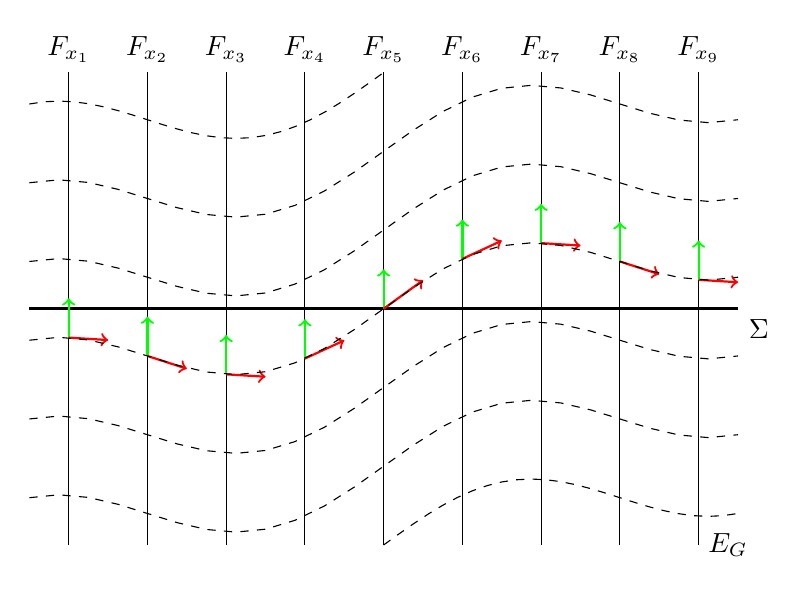
\begin{tikzpicture}[scale=0.5]
  \draw[very thick]
    (-9,0)
    --
    (9,0)
    node [below right] {$\Sigma$};
  \draw
    (-8,-6)
    --
    (-8,6)
    node [above] {$F_{x_{1}}$};
  \draw
    (-6,-6)
    --
    (-6,6)
    node [above] {$F_{x_{2}}$};
  \draw
    (-4,-6)
    --
    (-4,6)
    node [above] {$F_{x_{3}}$};
  \draw
    (-2,-6)
    --
    (-2,6)
    node [above] {$F_{x_{4}}$};
  \draw
    (0,-6)
    --
    (0,6)
    node [above] {$F_{x_{5}}$};
  \draw
    (2,-6)
    --
    (2,6)
    node [above] {$F_{x_{6}}$};
  \draw
    (4,-6)
    --
    (4,6)
    node [above] {$F_{x_{7}}$};
  \draw
    (6,-6)
    --
    (6,6)
    node [above] {$F_{x_{8}}$};
  \draw
    (8,-6)
    node [right] {$E_{G}$}
    --
    (8,6)
    node [above] {$F_{x_{9}}$};
  \draw[green,->,thick]
    (-8,{sin(-30*8)-8/5})
    --
    (-8,{sin(-30*8)-8/5+1});
  \draw[green,->,thick]
    (-6,{sin(-30*6)-6/5})
    --
    (-6,{sin(-30*6)-6/5+1});
  \draw[green,->,thick]
    (-4,{sin(-30*4)-4/5})
    --
    (-4,{sin(-30*4)-4/5+1});
  \draw[green,->,thick]
    (-2,{sin(-30*2)-2/5})
    --
    (-2,{sin(-30*2)-2/5+1});
  \draw[green,->,thick]
    (0,0)
    --
    (0,{sin(0)+1});
  \draw[green,->,thick]
    (2,{sin(30*2)+2/5})
    --
    (2,{sin(30*2)+2/5+1});
  \draw[green,->,thick]
    (4,{sin(30*4)+4/5})
    --
    (4,{sin(30*4)+4/5+1});
  \draw[green,->,thick]
    (6,{sin(30*6)+6/5})
    --
    (6,{sin(30*6)+6/5+1});
  \draw[green,->,thick]
    (8,{sin(30*8)+8/5})
    --
    (8,{sin(30*8)+8/5+1});
  \draw[red,->,thick]
    (-8,{sin(-30*8)-8/5})
    --
    ({-8+1},{30*pi*cos(-30*8)/180+1/5+sin(-30*8)-8/5});
  \draw[red,->,thick]
    (-6,{sin(-30*6)-6/5})
    --
    ({-6+1},{30*pi*cos(-30*6)/180+1/5+sin(-30*6)-6/5});
  \draw[red,->,thick]
    (-4,{sin(-30*4)-4/5})
    --
    ({-4+1},{30*pi*cos(-30*4)/180+1/5+sin(-30*4)-4/5});
  \draw[red,->,thick]
    (-2,{sin(-30*2)-2/5})
    --
    ({-2+1},{30*pi*cos(-30*2)/180+1/5+sin(-30*2)-2/5});
  \draw[red,->,thick]
    (0,0)
    --
    (1,{30*pi*cos(0)/180+1/5});
  \draw[red,->,thick]
    (2,{sin(30*2)+2/5})
    --
    ({2+1},{30*pi*cos(30*2)/180+1/5+sin(30*2)+2/5});
  \draw[red,->,thick]
    (4,{sin(30*4)+4/5})
    --
    ({4+1},{30*pi*cos(30*4)/180+1/5+sin(30*4)+4/5});
  \draw[red,->,thick]
    (6,{sin(30*6)+6/5})
    --
    ({6+1},{30*pi*cos(30*6)/180+1/5+sin(30*6)+6/5});
  \draw[red,->,thick]
    (8,{sin(30*8)+8/5})
    --
    ({8+1},{30*pi*cos(30*8)/180+1/5+sin(30*8)+8/5});
  \draw[dashed,domain=0:9]
    plot
    ({\x},{sin(30*\x)+\x/5-6});
  \draw[dashed,domain=-9:9]
    plot
    ({\x},{sin(30*\x)+\x/5-4});
  \draw[dashed,domain=-9:9]
    plot
    ({\x},{sin(30*\x)+\x/5-2});
  \draw[dashed,domain=-9:9]
    plot
    ({\x},{sin(30*\x)+\x/5});
  \draw[dashed,domain=-9:9]
    plot
    ({\x},{sin(30*\x)+\x/5+2});
  \draw[dashed,domain=-9:9]
    plot
    ({\x},{sin(30*\x)+\x/5+4});
  \draw[dashed,domain=-9:0]
    plot
    ({\x},{sin(30*\x)+\x/5+6});
\end{tikzpicture}
\]
The arrows in the picture hint at some equivalent characterizations of parallel transport. To understand this let us explain what the arrows mean. First of all, let us say that the green arrows parallel to the fibers should have been drawn at any crossing of fiber and dashed lines and not just for one of the dashed lines as well as the red arrows tangential to the dashed lines. For $e \in E_{G}$ let $T_{e}E_{G}$ denote the tangent space of $E_{G}$ at $e$.
\begin{enumerate}
\item[$\bullet$]
The green arrows should be understood symbolically as the subspace $V_{e}E_{G}$ of $T_{e}E_{G}$ which is tangential to the fiber, that is, the kernel of the tangent map $T_{e}\pi_{G} \colon T_{e}E_{G} \rightarrow T_{\pi_{G}(e)}\Sigma$ of $\pi_{G}$ (which is linear). $V_{e}E_{G}$ is referred to as vertical subspace and is independent of any parallel transport.
\item[$\bullet$]
The red arrows shall stand for the vector field on $E_{G}$ corresponding to the flow expressed by the dashed lines. So the red arrows are as good as the dashed lines here. Moreover we get dashed lines for any path in $\Sigma$ from a parallel transport and thus red arrows. All these red arrows at some $e \in E_{G}$ together span a subspace $H_{e}E_{G}$ of $T_{e}E_{G}$. $H_{e}E_{G}$ is referred to as horizontal subspace for the chosen parallel transport and hence depends on the chosen parallel transport. Moreover note that $H_{e}E_{G}$ gets along with the action on the fiber in the sense that the tangent map of the action maps horizontal spaces to horizontal spaces.
\end{enumerate}
What the picture now suggests is that given a parallel transport we have a direct sum decomposition
\begin{align*}
  T_{e}E_{G}
  &=
  V_{e}E_{G}
  \oplus
  H_{e}E_{G}
\end{align*}
such that the action on the fibers is respected. What we want to say is that instead of giving a parallel transport it suffices to (smoothly) specify $H_{e}E_{G}$ at each point of $E_{G}$ in a way that respects the action on the fiber.
\begin{enumerate}
\item[$\pmb{\hookrightarrow}$]
Mathematically, this smooth choice of horizontal space distribution is usually referred to as Ehresmann connection on $\pi_{G}$.
\end{enumerate}
This picture hopefully makes the terminology {\glqq}connection{\grqq} clear since it shall indicate how the fibers are {\glqq}connected{\grqq}. There is a convenient way to specify an Ehresmann connection. To this end consider the tangent bundles $\pi_{TE_{G}} \colon TE_{G} \rightarrow E_{G}$ and $\pi_{T\Sigma} \colon T\Sigma \rightarrow \Sigma$ on $E_{G}$ and $\Sigma$, respectively. We then have the vector bundle homomorphism
\begin{align*}
  T\pi_{G}
  :=
  (T_{e}\pi_{G})
  \colon
  TE_{G}
  &\rightarrow
  T\Sigma
\end{align*}
from $\pi_{G} \circ \pi_{TE_{G}}$ to $\pi_{T\Sigma}$ induced by the tangent maps $T_{e}\pi_{G}$. Now note that under factoring out the fiberwise action by $G$ from $E_{G}$ we get a unique vector bundle $\pi_{TE_{G}}^{!} \colon TE_{G} \slash G \rightarrow \Sigma$ with total space the quotient. Moreover the vector bundle homomorphism $T\pi_{G}$ induces a unique vector bundle homomorphism
\begin{align*}
  T\pi_{G}^{!}
  \colon
  TE_{G}
  \slash
  G
  &\rightarrow
  T\Sigma
\end{align*}
from $\pi_{TE_{G}}^{!}$ to $\pi_{T\Sigma}$. Now a smooth section $\sigma$ of $T_{e}\pi_{G}$ which is linear, that is, a linear map
\begin{align*}
  \sigma
  \colon
  T_{\pi_{G}(e)}\Sigma
  &\rightarrow
  T_{e}E_{G}
\end{align*}
such that $T_{e}\pi_{G} \circ \sigma$ is the identity, can be shown to already determine a horizontal subspace using the fact that $\sigma$ as linear section maps only the $0$ to the vertical subspace. Moreover, because it essentially suffices to determine one horizontal subspace in each fiber due to the compatibility with the action, an Ehresmann connection on $\pi_{G}$ can be seen to correspond precisely to a smooth section of $T\pi_{G}^{!}$, considered as homomorphism of vector bundles. So to define an Ehresmann connection on $\pi_{G}$ we can provide a certain family of linear maps
\begin{align*}
  \sigma_{x}
  \colon
  T_{x}\Sigma
  &\rightarrow
  \left(
    \pi_{TE_{G}}^{!}
  \right)^{-1}
  (x)
\end{align*}
smoothly depending on $x$. In other words: an Ehresmann connection is nothing but a smooth section of the \textit{homomorphism bundle for $\pi_{G}$} which is just the tensor bundle
\begin{align*}
  \pi_{T\Sigma}^{\prime}
  \otimes
  \pi_{TE_{G}}^{!}
  \colon
  E_{\pi_{G}}
  &\rightarrow
  \Sigma
\end{align*}
where $\pi_{T\Sigma}^{\prime}$ is the fiberwise vector space dual to $\pi_{T\Sigma}$ and $\sigma_{x}$ is then an element (up to isomorphism from tensoring) of a fiber of this bundle. So a connection can be regarded as a section of a fiber bundle. Namely one with fiber the vector space of some vector space homomorphisms. But there is still another convenient characterization of the idea described so far. This arises from the Ehresmann connection in the following way. Because $V_{e}E_{G}$ is regarded as being tangential to the fiber and the fiber is isomorphic to the Lie group $G$ the vertical subspace $V_{e}E_{G}$ should be isomorphic to the Lie algebra $\mathrm{Lie}_{G}$ of $G$ which is by definition just the tangent space at the identity element of the Lie group. Given an Ehresmann connection we can now map any vector in $T_{e}E_{G}$ to its $V_{e}E_{G}$ component such that this function gets along with the action in some sense. What we then get in the end is essentially a Lie algebra-valued $1$-form subjected to some properties.
\begin{enumerate}
\item[$\pmb{\hookrightarrow}$]
Mathematically, this Lie algebra-valued $1$-form with its properties is usually referred to as principal connection on $\pi_{G}$.
\end{enumerate}
For the record:
\begin{enumerate}
\item[$\pmb{\hookrightarrow}$]
Mathematically, we have an equivalence of
\begin{enumerate}
\item[$\bullet$]
Parallel Transport for $\pi_{G}$
\item[$\bullet$]
Ehresmann Connection on $\pi_{G}$
\item[$\bullet$]
Principal Connection on $\pi_{G}$
\end{enumerate}
This equivalence can be found to some extent in \cite{797789bc}. More on this (including sources) can also be found in \cite{wiki-nlab0000}: connection on a bundle.
\end{enumerate}
Note that whenever we are given an action $\mathrm{a}_{F}$ of $G$ on a smooth manifold $F$ then we can loosely speaking replace each fiber $F_{x}$ of $\pi_{G}$ by $F$ to get a fiber bundle $\pi_{\mathrm{a}_{F}}$ over $\Sigma$. And then each parallel transport induces such a notion in $\pi_{\mathrm{a}_{F}}$. If further $F$ is a vector space this parallel transport allows to define a differential quotient.
\begin{enumerate}
\item[$\pmb{\hookrightarrow}$]
Mathematically, we are talking about the bundle associated with $\pi_{G}$ via an action of $G$ on $F$ and in case of $F$ a vector space the covariant derivative for the parallel transport. The covariant derivative in an associated vector bundle is a coordinate free way of measuring change of sections in this bundle along vector fields. Details can be found in \cite{797789bc}.
\end{enumerate}
So whenever we have sections of a vector bundle associated with a principal bundle governing a local symmetry we should use the covariant derivative w.r.t. this symmetry when we have to determine the change of such a section in spacetime to get along with the symmetry. Now as it is instructive to understand a manifold in local coordinates we expect this to be interesting in the case of a bundle, too. So let $s \colon U \rightarrow E_{G}$ be a smooth local section of the $G$-principal bundle $\pi_{G}$ on which we have a principal connection $\omega$. We can use the tangent map of $s$ to map a tangent vector of $U$ to one of $E_{G}$ to which we can then apply $\omega$ to get a vector in the Lie algebra. So, locally, we expect to get a Lie algebra-valued $1$-form $s^{\ast}(\omega)$ on $U$ from $\omega$ depending on the chosen section $s$. And choosing coordinates $q_{\varphi}^{i}$ for $U$ we can write
\begin{align*}
  s^{\ast}(\omega)(x)
  &=
  \sum_{i=0}^{n}
  A_{q_{\varphi}^{i}}^{s}(x)
  \mathrm{d}q_{\varphi}^{i}(x)
\end{align*}
here with functions $A_{q_{\varphi}^{i}}^{s} \colon U \rightarrow \mathrm{Lie}_{G}$ (depending on the choice of $s$).
\begin{enumerate}
\item[$\pmb{\hookrightarrow}$]
Mathematically, $s^{\ast}(\omega)$ is the pullback of $\omega$ along $s$ and this can be regarded as a smooth local section of the cotangent bundle tensored with the Lie algebra of $G$ which then i.p. results in a vector bundle.
\end{enumerate}
This is a neat simplification of the connection (locally) and it is an interesting question if we can reconstruct $\omega$ from such local data on $\Sigma$. So assuming a set $K$ and smooth local sections $s_{k} \colon U_{k} \rightarrow E_{G}$ of $\pi_{G}$ for all $k \in K$ trivializing all of $\pi_{G}$ this is to say: can we reconstruct $\omega$ from all the local Lie algebra-valued one forms $s_{k}^{\ast}(\omega)$ on $U_{k}$? To answer this question it seems that one should understand what happens on $U_{k_{1}} \cap U_{k_{2}}$ for $(k_{1},k_{2}) \in K \times K$. So we should stick with the coordinate approach and see what a change of local coordinates does. First note that for smooth local sections $s_{1} \colon U_{1} \rightarrow E_{G}$ and $s_{2} \colon U_{2} \rightarrow E_{G}$ of $\pi_{G}$ we have for each $x \in U_{k_{1}} \cap U_{k_{2}}$ a unique $g_{x} \in G$ such that
\begin{align*}
  s_{2}(x)
  &=
  \mathrm{a}_{x}
  \left(
    g_{x},
    s_{1}(x)
  \right)
\end{align*}
due to the free transitivity of the action $\mathrm{a}_{x}$ on the fiber $F_{x}$ of $\pi_{G}$. Then the change of coordinates from $s_{1}$ to $s_{2}$ corresponds precisely to the smooth function
\begin{align*}
  \tau_{s_{1},s_{2}}
  \colon
  U_{k_{1}}
  \cap
  U_{k_{2}}
  &\rightarrow
  G
  \\
  x
  &\mapsto
  g_{x}
\end{align*}
called transition function. Moreover note that there is an explicit formula - let us label this $\mathfrak{F}_{q_{\varphi}^{i}}^{s_{1},s_{2}}(\omega)$ for the sake of easy reference here - relating $A_{q_{\varphi}^{i}}^{s_{1}}(x)$ and $A_{q_{\varphi}^{i}}^{s_{2}}(x)$ for all $x \in U_{1} \cap U_{2}$ using the transition function $\tau_{s_{1},s_{2}}$. For details see \cite{797789bc}. However, we will later write this formula down in the case of matrix groups. Now back to the trivializing sections $s_{k}$. Then for all pairs $(k_{1},k_{2}) \in K \times K$ we have transition functions $\tau_{s_{k_{1}},s_{k_{2}}}$ and these satisfy the cocycle condition\footnote{yes this has to do with cohomology as we will see more explicitly later in chapter \ref{chap:cattg}}
\begin{align*}
  \tau_{s_{k_{1}},s_{k_{2}}}(x)
  \cdot
  \tau_{s_{k_{2}},s_{k_{3}}}(x)
  &=
  \tau_{s_{k_{1}},s_{k_{3}}}(x)
\end{align*}
for all suited $x$ and all possible combinations of $k_{1},k_{2},k_{3} \in K$. This in particular implies
\begin{align*}
  \tau_{s_{k},s_{k}}(x)
  &=
  e_{G}
  \\
  \tau_{s_{k_{1}},s_{k_{2}}}(x) 
  &=
  \tau_{s_{k_{2}},s_{k_{1}}}(x)^{-1}
\end{align*}
where $e_{G}$ denotes the identity element of $G$. One can show that from this data - the transition functions satisfying the cocycle condition - $\pi_{G}$ is reconstructable up to isomorphism. One can even show that functions $A_{q_{\varphi}^{i}}^{s_{k}} \colon U_{k} \rightarrow \mathrm{Lie}_{G}$ pairwise related by $\mathfrak{F}_{q_{\varphi}^{i}}^{s_{k_{1}},s_{k_{2}}}(\omega)$ on overlaps patch together to a unique connection on $\pi_{G}$. So the $s_{k}^{\ast}(\omega)$ already determine the connection. Now assume further smooth local sections $s_{k}^{\backprime} \colon U_{k} \rightarrow E_{G}$ of $\pi_{G}$ for all $k \in K$ trivializing all of $\pi_{G}$. Then there are unique smooth functions
\begin{align*}
  f_{s_{k},s_{k}^{\backprime}}
  \colon
  U_{k}
  &\rightarrow
  G
\end{align*}
satisfying the coboundary condition
\begin{align*}
  f_{s_{k_{1}},s_{k_{1}}^{\backprime}}(x)
  \cdot
  \tau_{s_{k_{1}}^{\backprime},s_{k_{2}}^{\backprime}}(x)
  &=
  \tau_{s_{k_{1}},s_{k_{2}}}(x)
  \cdot
  f_{s_{k_{2}},s_{k_{2}}^{\backprime}}(x)
\end{align*}
for all suited $x$. One can then show that the bundle reconstructed from the $s_{k}$ is isomorphic to the bundle reconstructed from the $s_{k}^{\backprime}$ using the $f_{k}$ satisfying the coboundary condition. This in particular shows that a change of coordinates from $s_{k}$ to $s_{k}^{\prime}$ originates from a $G$-principle bundle isomorphism $\Phi$ from $\pi_{G}$ to $\pi_{G}$. Note that the pullback $\Phi^{\ast}(\omega)$ of a principal connection $\omega$ is also a principal connection. And the connection $\Phi^{\ast}(\omega)$ in the coordinates $s_{k}$ is the same as $\omega$ in coordinates $\Phi \circ s_{k}$.\footnote{this is since pulling back essentially respects composition contravariantly as you will know after chapter \ref{chap:cattg}} On the other hand, $f_{s_{k},s_{k}^{\backprime}}$ is what we actually wanted as change of perspective respecting the principle of locality. So in the end, if we change local coordinates of the physical situation we are looking at we must change local coordinates of the connection at the same time. The common ground of these changes is the isomorphism $\Phi$. Thus it seems better to regard the isomorphisms of the bundle as actual changes of perspective. Let us run through an easy class of examples which cover most physically relevant cases. Namely $G$ as a sub Lie group of the $n$-dimensional general linear group $GL(n,\mathbb{K})$ with coefficients in $\mathbb{K} = \mathbb{R},\mathbb{C}$. The Lie algebra $\mathrm{Lie}_{G}$ is then also a matrix group and for an isomorphism $\Phi$ and local coordinates $s$ we have
\begin{align*}
  (\Phi \circ s)(x)
  &=
  \tau_{s,\Phi \circ s}(x)
  \cdot
  s(x)
  \\
  A_{q_{\varphi}^{i}}^{\Phi \circ s}(x)
  &=
  \tau_{s,\Phi \circ s}(x)
  \cdot
  A_{q_{\varphi}^{i}}^{s}(x)
  \cdot
  \tau_{s,\Phi \circ s}(x)^{-1}
  +
  \tau_{s,\Phi \circ s}(x)
  \cdot
  \partial_{q_{\varphi}^{i}(x)}
  \tau_{s,\Phi \circ s}(x)^{-1}
\end{align*}
according to \cite{797789bc}. In particular, for $G = U(1)$ the $1$-dimensional unitary group, which geometrically as a manifold is nothing but a circle, the Lie algebra $\mathrm{Lie}_{U(1)}$ is isomorphic to $\mathbb{R}$ as vector space and we have
\begin{align*}
  (\Phi \circ s)(x)
  &=
  \mathrm{exp}(\mathrm{i}\theta_{\Phi}(x))
  \cdot
  s(x)
  \\
  A_{q_{\varphi}^{i}}^{\Phi \circ s}(x)
  &=
  A_{q_{\varphi}^{i}}^{s}(x)
  +
  \partial_{q_{\varphi}^{i}(x)}
  \theta_{\Phi}(x)^{-1}
\end{align*}
Moreover for the action
\begin{align*}
  \mathrm{a}_{\mathbb{C}^{n}}
  \colon
  U(1)
  \times
  \mathbb{C}^{n}
  &\rightarrow
  \mathbb{C}^{n}
  \\
  (\mathrm{exp}(\mathrm{i}\theta),z)
  &\mapsto
  \mathrm{exp}(\mathrm{i}\theta)
  \cdot
  z
\end{align*}
where $\cdot$ means scalar multiplication and a smooth section $\phi$ of the vector bundle $\pi_{\mathbb{C}^{n}}$ associated with $\pi_{U(1)}$ via $\mathrm{a}_{\mathbb{C}^{n}}$ the covariant derivative $D_{q_{\varphi}^{i}(x)}^{s}$ of $\phi$ in the chosen coordinates is given by
\begin{align*}
  \left(
    D_{q_{\varphi}^{i}(x)}^{s}
    \phi
  \right)
  (x)
  &=
  \left(
    \partial_{q_{\varphi}^{i}(z)}
    \phi
  \right)
  (x)
  +
  A_{q_{\varphi}^{i}}^{s}(x)
  \cdot
  \phi(x)
\end{align*}
Let us summerize what we have done here. We proposed a mathemtical description of a physical situation which is the same under different viewpoints and respects the principle of locality. Then from the desire to compare for changes at near points in spacetime we predicted the need of a section of some fiber bundle (namely the connection $\omega$) from purely geometrical considerations. And the view on this section depends on the view on the physical situation. So one might conjecture that this section is somehow influenced (at least) by the sole presence of the physical situation.
\item[(4)]
Physical quantities are often described as things on spacetime. Just think of
\begin{enumerate}
\item[$\bullet$]
semi-Riemannian metrics in GR
\item[$\bullet$]
potentials in electrodynamics\footnote{usually only for $\Sigma = \mathbb{R}^{4}$ as Minkowski spacetime but possibly also on arbitrary spacetimes}
\item[$\bullet$]
wave functions in relativistic quantum mechanics\footnote{usually only for $\Sigma = \mathbb{R}^{4}$ Minkowski spacetime} (Klein-Gordon and Dirac equation)
\end{enumerate}
which already covers a significant part of traditional\footnote{from the first half of the 20th century} physics. We go into more detail in a moment. But first some terminological settlements. The physical quantities we are talking about are usually called fields or field configurations and one can take the stance that (theoretical) physics is all about the description of fields from a nowadays perspective.
\begin{enumerate}
\item[$\pmb{\hookrightarrow}$]
Mathematically, a field should be smooth section of a smooth fiber bundle\footnote{we assume those locally trivial by definition} over spacetime $\Sigma$.
\end{enumerate}
In physics, one calls a fiber bundle over spacetime
\begin{align*}
  \pi
  \colon
  E_{\pi}
  &\rightarrow
  \Sigma
\end{align*}
with fiber $F_{\pi}$ field bundle while the fiber of this bundle is called field fiber and is often denoted $\mathrm{Conf}_{\pi} := F_{\pi}$. The space of smooth sections of the bundle $\pi$ is denoted
\begin{align*}
  \Gamma_{\pi}^{\mathrm{glob}}
\end{align*}
and called field configuration space. A point of this space is consequently called a field configuration. If $U$ is a subspace of $\Sigma$ then we have a smooth fiber bundle
\begin{align*}
  \pi
  \vert
  U
  \colon
  \pi^{-1}(U)
  &\rightarrow
  U
  \\
  e
  &\mapsto
  \pi(e)
\end{align*}
and hence we can define
\begin{align*}
  \Gamma_{\pi}(U)
  &:=
  \Gamma_{\pi \vert U}^{\mathrm{glob}}
\end{align*}
which are the local sections of $\pi$ over $U$ and are called local field configurations. The principle of locality suggets that for any cover of $\Sigma$ by subspaces we should be able to uniquely construct a field configuartion from local ones which match on overlaps.
\begin{enumerate}
\item[$\pmb{\hookrightarrow}$]
Mathematically, this means that $\Gamma_{\pi}$ should be something like a sheaf\footnote{a not so small part of chapter \ref{chap:cattg} is ultimately about sheaves (including motivation and a formal definition)}.
\end{enumerate}
So what actually matters when we demand the principal of locality is $\Gamma_{\pi}$ and not so much the field bundle. Note that if moreover $U$ is such that $\pi$ is trivial over it then restricting a field configuration from $\Gamma_{\pi}^{\mathrm{glob}}$ to $U$ can be considered a function from $U$ to $\mathrm{Conf}_{\pi}$ since
\begin{align*}
  (\pi \vert U)^{-1}(U)
  &\cong
  U
  \times
  \mathrm{Conf}_{\pi}
\end{align*}
And if we even have charts with domain $U$ then, locally, a field configuration can be considered a function from $\mathbb{R}^{n+1}$ to $\mathrm{Conf}_{\pi}$. Note that fields are often defined as such functions or perhaps more generally as functions from $\Sigma$ to $\mathrm{Conf}_{\pi}$. In our language this is to say that fields are defined to be trivial bundles. While this is appropriate for electrodynamics and relativistic quantum mechanics to some extent it does not make sense for GR whose metric is a tensorfield over spacetime which is a section of a certain fiber bundle in general. Anyways, the interpretation of fields as sections through bundles implies that connections on principal bundles are fields since they can be regarded as sections through the homomorphism bundle
\begin{align*}
  \pi_{T\Sigma}^{\prime}
  \otimes
  \pi_{TE_{G}}^{!}
  \colon
  E_{\pi_{G}}
  &\rightarrow
  \Sigma
\end{align*}
from above. This qualifies the connections to have a physical meaning which even seems natural since we predicted them from a physical desire. And not only this, we can patch the connection $\omega$ together from local fields $s_{k}^{\ast}(\omega)$ when we track the symmetry transformations. However, we lack an interpretation so far. So let us look at our initial examples of point (3). Both of these are a bit unrealistic in the light of GR and relativistic quantum mechanics. So let us take a closer look.
\begin{enumerate}
\item[$\bullet$]
In GR we do not only assume spacetime to be a smooth manifold but we also assume a semi-Riemannian metric on it among other things. And this demand has to be compatible with general covariance. In the end one is more or less forced to take the Levi-Civita connection on the frame bundle $\pi_{GL(n+1)}$ over spacetime $\Sigma$ for the purpose of GR. This connection is uniquely determined by the semi-Riemannian metric. So the covariant derivative of GR in any associated bundle (i.p. tensor bundles) is the one obtained from the Levi-Civita connection. In GR all relevant fields are sections of such associated bundles. The $A_{q_{\varphi}^{i}}^{s}(x)$ are known as Christoffel symbols. Note that if we take $\Sigma = \mathbb{R}^{4}$ as Minkowski spacetime we get the ordinary derivative from the Levi-Civita connection since we have global sections of the principal bundle in this case.
\item[$\bullet$]
If anything is a field on spacetime then also a massive particle with internal symmetry ought to be so. So take a relativistic electron with spin $\psi \colon \mathbb{R}^{4} \rightarrow \mathbb{C}^{4}$ as solution of the Dirac equation, for example. This can be regarded as a section of the bundle associated to the trivial $U(1)$-bundle via $\mathrm{a}_{\mathbb{C}^{4}}$ from point (3). Now the electron must influence the connection and the obvious thing an electron influences is the electromagnetic field. But the electromagnetic field is a $2$-form while the connection is a Lie alegebra-valued $1$-form here. However, the potential of the electromagnetic field can be considered as such. So one might conjecture that the predicted section (the connection) is the potential generated by the electron. This is further underpinned by the behaviour of $A_{q_{\varphi}^{i}}^{s}$ under symmetry transformations. But note that the Maxwell equations for the potential have vacuum solutions and one has to take these into account for the connection, too, then. This is the idea of quantum electrodynamics (abbr. QED). More generally, this suggests that a massive particle with internal symmetry a Lie group $G$ is a section of a bundle associated with a $G$-principal bundle over Minkowski spacetime governing the symmetry while the connections on this bundle are the fields of the potential of the predicted fundamental force which also has vacuum solutions. This idea was very successful in that three of the four known fundamental forces (all but the gravitational force) were combined into the SMP with a single Lie group $G_{\textrm{SMP}}$. So to understand the SMP locally we have to look at $G_{\textrm{SMP}}$-principal bundles over Minkowski spacetime and connections on it. But we want to understand it globally so we should look at principal bundles over any spacetime $\Sigma$ and connections on it, as well as sections through associated bundles and their covariant derivatives in case of vector bundles.
\end{enumerate}
Physically, a major reason of why to take arbitrary principle bundles into account (and hence a further reason for arbitrary field bundles) is that the principal bundle twists encode the theoretically important \textit{instantons} which are for instance relevant to understand the vacuum state of the SMP. The bundle twists depend only on the isomorphism class of the principal bundle and people are tempted to factor isomorphism out. This thinking arises from an often unrecognized misconception regarding symmetry and redundancy. On the philosophical level: symmetry is not the same as redundancy. Symmetry means that we can look at a situation from different perspectives without observing a difference in the situation but this does not imply that we can identify these perspectives with each other to one single perspective. This would collapse the symmetry information and we would hence lose information which we would not if we had redundancy. The physical argument against this is that if we collapse the symmetry information then we can only regain $\omega$ from the local data $s_{k}^{\ast}(\omega)$ if $\pi_{G}$ is trivial and hence allows for a (global) smooth section. So we would have to give up the principle of locality or instantons. Or we just allow to track the symmetry in the definition of field. This is to say that we map any patch $U$ of spacetime to the collection of $G$-principle bundles over $U$ with connection structured by bundle isomorphisms preserving the connection. Additionally, we require that we can uniquely glue things together on overlaps.
\begin{enumerate}
\item[$\pmb{\hookrightarrow}$]
Mathematically, the structured collection is a groupoid - which is actually a homotopy $1$-type - while mapping the patches to these groupoids under such a condition is a stack (kind of a weakened sheaf in some sense usually expressed as groupoid-valued functor). If one develops this idea further with symmetry of symmetry\footnote{this can be important in string theory} and so on then one ends up with $\infty$-groupoids - which capture the full homotopy of topological spaces (Grothendieck hypothesis) - and $\infty$-stacks (kind of sheaf up to homotopy in some sense usually expressed as $\infty$-groupoid-valued functor). So it seems reasonable to model physical fields obeying the principle of locality as $\infty$-stacks.
\end{enumerate}
For more on this see \cite{d1ad46b9} and \cite{wiki-nlab0000}: field (physics). After all we see that homotopy theory and category theory\footnote{e.g. the functors here} are important in physics. But stacks are not the only point where homotopical properties matter in physics. For instance, the parallel transport depends on the homotopy class of the path. And the Berry phase of an electron we mentioned earlier has its origin in an electron moving around a homotopically non-trivial path. But homotopy theory has much to do with category theory as we hinted earlier and so we have another way how category theory becomes important to physics. And this is still not all: Let $X$ be a CW complex then - when we require only continuous instead of smooth - an isomorphism class of $G$-principal bundles over $X$ corresponds precisely to a homotopy class of maps from $X$ to a CW complex $\mathrm{B}G$ obtained from $G$ which in turn corresponds to a cohomology class in the first cohomology\footnote{singular if $G$ is abelian} group with coefficients in $G$.\footnote{for the latter we should take basepoints into account} We write this boldly as
\begin{align*}
  \mathcal{P}_{G}(X)
  &\cong
  \mathrm{hom}_{\mathrm{Ho}(\mathbf{Top}_{\ast}^{\textrm{CW}})}
  \left(
    X,
    \mathrm{B}G
  \right)
  \cong
  h_{G}^{1}(X)
\end{align*}
It needs much of chapter \ref{chap:cattg} to understand this categorically even though we do not really prove it in full generality. Unfortunately, this classification does not work for isomorphism classes of principle bundles over a manifold with connection. But there is a way around this by replacing smooth manifolds with a more general kind of space. These generalized spaces will be a recurring example in chapter \ref{chap:cattg}. The only problem left are then the isomorphism classes where we actually should use higher groupoids.
\item[(5)]
The physical laws which govern the field configuration can often be obtained from a Lagrangian density for the field configuration by Hamilton's principle. Examples include:
\begin{enumerate}
\item[$\bullet$]
Einstein's field equations for semi-Riemannian metrics in GR
\item[$\bullet$]
Maxwell's equations for potentials in electrodynamics\footnote{usually only on Minkowski spacetime}
\item[$\bullet$]
Klein-Gordon and Dirac equation for wave functions in relativistic quantum mechanics\footnote{usually only on Minkowski spacetime}
\end{enumerate}
So the Lagrangian density for the field is assumed to contain much (if not all) information about the considered physical system. But one has to take care to take the right covariant derivative if necessary to incorporate the right local symmetry into the Lagrangian. For example, the QED Lagrangian on Minkowski spacetime is the sum of the vacuum electrodynamics Lagrangian and the Dirac Lagrangian where the latter uses the covariant derivative w.r.t. the symmetry of the electron which then results in an interaction of electron and electromagnetic field. Moreover note that if one further wants to incorporate the principal of locality here then the Lagrangian density for the field on a local patch of spacetime should in some way be independent of that on some disjoint patch. So one should actually take the local Lagrangian density.
\begin{enumerate}
\item[$\pmb{\hookrightarrow}$]
Mathematically, this is modelled as a horizontal differential form of degree the dimension of spacetime on the jet-bundle for the field bundle.
\end{enumerate}
We do not explain here what this is. Let us just say that, locally, on $U$ one gets what one would usually understand as Lagrangian density.
\end{enumerate}
So far we have actually only taken GR into acount but not quantum theory which is also a pillar of physics. To incorporate quantum theory one has to quantize the classical fields we described so far. This is one of the main problems of physics at the moment. One wants to find a process of getting a formal quantum field theory (abbr. QFT) from the classical field theory (fields and local Lagrangian densities) such as Feynman's path intgrals which are quite succesful but not mathematically rigorous. The processes of quantization are more thoroughly discussed in \cite{00000011}. There are essentially two mathematical approaches for formal QFTs: algebraic quantum field theory (abbr. AQFT) and functorial quantum field theory (abbr. FQFT).
\begin{enumerate}
\item[$\bullet$]
AQFT is the approach preferred by most mathematical physicists. The idea is to cover spacetime by subspaces each coming with an operator algebra made up by the observable physical quantities on this subspace. On overlaps the observables are expected to get along with each other in some sense. There are two well-known proposals for axiomatizations.\footnote{we want to emphasize the word {\glqq}proposal{\grqq} here} The Wightman axioms and the Haag-Kastler axioms, respectively. We do not want to go into detail here. We do not further discuss AQFTs here at all. We only want to say that the connection to category theory does not look so deep here. At least at first glance at which it seems as category theory would only provide a convenient language in some places in the guise of presheaves. Presheaves will play a major role in chapter \ref{chap:cattg} as you will see.
\item[$\bullet$]
FQFT is the approach which is obviously pure category theory. An FQFT is a (higher) {\glqq}functor{\grqq} from a certain geometric (higher) category to a certain algebraic (higher) category. A (higher) functor can be understood as higher-dimensional function if higher categories are considered higher dimensional sets. This is to say if a higher category is made up by countably many levels then a higher functor maps levels of some rank to levels of the same rank. If you do not understand this yet we guarantee you will after reading chapter \ref{chap:cattg}. Unfortunately, it is not yet known what the correct categories are. While the geometric domain category has to do with cobordisms as is more or less clear the algebraic one makes more problems. But there is a special case which is better understood: topological quantum field theory (abbr. TQFT). These are quantum field theories not depending on the metric of spacetime but rather on the geometry of it. TQFTs are a sort of reasonably formalized FQFTs. We will roughly sketch what a TQFT categorically is in chapter \ref{chap:cattg} but then refer to \cite{00000011} which precisely defines them together with a motivation from Feynman's path integrals.
\end{enumerate}
AQFT and FQFT can be understood as dual\footnote{roughly: the same from different perspectives} to each other in the sense that algebra and geometry can be understood as dual to each other.\footnote{This is captured by so-called Isbell duality in category theory and can be traced back to Grothendiecks functorial geometry over Lawvere's idea of a duality of generalized space - a recurring example in chapter \ref{chap:cattg} and quantity. However, we will neither prove nor state Isbell duality in these notes.} In physics this manifests itself in the Heisenberg picture which is known as the algebraic point of view on quantum mechanics and the Schr\"odinger picture which is known as the geometric point of view on quantum mechanics.
\\\\
Finally note, that in \cite{wiki-nlab0000} they more or less say a gauge theory is a \textit{QFT} whose \textit{field configurations} are \textit{principal bundles with connection}. So this section was ultimately all about higher category in gauge theory which is a dominant field of research in modern physics.
